% Options for packages loaded elsewhere
% Options for packages loaded elsewhere
\PassOptionsToPackage{unicode}{hyperref}
\PassOptionsToPackage{hyphens}{url}
\PassOptionsToPackage{dvipsnames,svgnames,x11names}{xcolor}
%
\documentclass[
  letterpaper,
  DIV=11,
  numbers=noendperiod]{scrartcl}
\usepackage{xcolor}
\usepackage[margin=1in]{geometry}
\usepackage{amsmath,amssymb}
\setcounter{secnumdepth}{5}
\usepackage{iftex}
\ifPDFTeX
  \usepackage[T1]{fontenc}
  \usepackage[utf8]{inputenc}
  \usepackage{textcomp} % provide euro and other symbols
\else % if luatex or xetex
  \usepackage{unicode-math} % this also loads fontspec
  \defaultfontfeatures{Scale=MatchLowercase}
  \defaultfontfeatures[\rmfamily]{Ligatures=TeX,Scale=1}
\fi
\usepackage{lmodern}
\ifPDFTeX\else
  % xetex/luatex font selection
\fi
% Use upquote if available, for straight quotes in verbatim environments
\IfFileExists{upquote.sty}{\usepackage{upquote}}{}
\IfFileExists{microtype.sty}{% use microtype if available
  \usepackage[]{microtype}
  \UseMicrotypeSet[protrusion]{basicmath} % disable protrusion for tt fonts
}{}
\makeatletter
\@ifundefined{KOMAClassName}{% if non-KOMA class
  \IfFileExists{parskip.sty}{%
    \usepackage{parskip}
  }{% else
    \setlength{\parindent}{0pt}
    \setlength{\parskip}{6pt plus 2pt minus 1pt}}
}{% if KOMA class
  \KOMAoptions{parskip=half}}
\makeatother
% Make \paragraph and \subparagraph free-standing
\makeatletter
\ifx\paragraph\undefined\else
  \let\oldparagraph\paragraph
  \renewcommand{\paragraph}{
    \@ifstar
      \xxxParagraphStar
      \xxxParagraphNoStar
  }
  \newcommand{\xxxParagraphStar}[1]{\oldparagraph*{#1}\mbox{}}
  \newcommand{\xxxParagraphNoStar}[1]{\oldparagraph{#1}\mbox{}}
\fi
\ifx\subparagraph\undefined\else
  \let\oldsubparagraph\subparagraph
  \renewcommand{\subparagraph}{
    \@ifstar
      \xxxSubParagraphStar
      \xxxSubParagraphNoStar
  }
  \newcommand{\xxxSubParagraphStar}[1]{\oldsubparagraph*{#1}\mbox{}}
  \newcommand{\xxxSubParagraphNoStar}[1]{\oldsubparagraph{#1}\mbox{}}
\fi
\makeatother

\usepackage{color}
\usepackage{fancyvrb}
\newcommand{\VerbBar}{|}
\newcommand{\VERB}{\Verb[commandchars=\\\{\}]}
\DefineVerbatimEnvironment{Highlighting}{Verbatim}{commandchars=\\\{\}}
% Add ',fontsize=\small' for more characters per line
\usepackage{framed}
\definecolor{shadecolor}{RGB}{241,243,245}
\newenvironment{Shaded}{\begin{snugshade}}{\end{snugshade}}
\newcommand{\AlertTok}[1]{\textcolor[rgb]{0.68,0.00,0.00}{#1}}
\newcommand{\AnnotationTok}[1]{\textcolor[rgb]{0.37,0.37,0.37}{#1}}
\newcommand{\AttributeTok}[1]{\textcolor[rgb]{0.40,0.45,0.13}{#1}}
\newcommand{\BaseNTok}[1]{\textcolor[rgb]{0.68,0.00,0.00}{#1}}
\newcommand{\BuiltInTok}[1]{\textcolor[rgb]{0.00,0.23,0.31}{#1}}
\newcommand{\CharTok}[1]{\textcolor[rgb]{0.13,0.47,0.30}{#1}}
\newcommand{\CommentTok}[1]{\textcolor[rgb]{0.37,0.37,0.37}{#1}}
\newcommand{\CommentVarTok}[1]{\textcolor[rgb]{0.37,0.37,0.37}{\textit{#1}}}
\newcommand{\ConstantTok}[1]{\textcolor[rgb]{0.56,0.35,0.01}{#1}}
\newcommand{\ControlFlowTok}[1]{\textcolor[rgb]{0.00,0.23,0.31}{\textbf{#1}}}
\newcommand{\DataTypeTok}[1]{\textcolor[rgb]{0.68,0.00,0.00}{#1}}
\newcommand{\DecValTok}[1]{\textcolor[rgb]{0.68,0.00,0.00}{#1}}
\newcommand{\DocumentationTok}[1]{\textcolor[rgb]{0.37,0.37,0.37}{\textit{#1}}}
\newcommand{\ErrorTok}[1]{\textcolor[rgb]{0.68,0.00,0.00}{#1}}
\newcommand{\ExtensionTok}[1]{\textcolor[rgb]{0.00,0.23,0.31}{#1}}
\newcommand{\FloatTok}[1]{\textcolor[rgb]{0.68,0.00,0.00}{#1}}
\newcommand{\FunctionTok}[1]{\textcolor[rgb]{0.28,0.35,0.67}{#1}}
\newcommand{\ImportTok}[1]{\textcolor[rgb]{0.00,0.46,0.62}{#1}}
\newcommand{\InformationTok}[1]{\textcolor[rgb]{0.37,0.37,0.37}{#1}}
\newcommand{\KeywordTok}[1]{\textcolor[rgb]{0.00,0.23,0.31}{\textbf{#1}}}
\newcommand{\NormalTok}[1]{\textcolor[rgb]{0.00,0.23,0.31}{#1}}
\newcommand{\OperatorTok}[1]{\textcolor[rgb]{0.37,0.37,0.37}{#1}}
\newcommand{\OtherTok}[1]{\textcolor[rgb]{0.00,0.23,0.31}{#1}}
\newcommand{\PreprocessorTok}[1]{\textcolor[rgb]{0.68,0.00,0.00}{#1}}
\newcommand{\RegionMarkerTok}[1]{\textcolor[rgb]{0.00,0.23,0.31}{#1}}
\newcommand{\SpecialCharTok}[1]{\textcolor[rgb]{0.37,0.37,0.37}{#1}}
\newcommand{\SpecialStringTok}[1]{\textcolor[rgb]{0.13,0.47,0.30}{#1}}
\newcommand{\StringTok}[1]{\textcolor[rgb]{0.13,0.47,0.30}{#1}}
\newcommand{\VariableTok}[1]{\textcolor[rgb]{0.07,0.07,0.07}{#1}}
\newcommand{\VerbatimStringTok}[1]{\textcolor[rgb]{0.13,0.47,0.30}{#1}}
\newcommand{\WarningTok}[1]{\textcolor[rgb]{0.37,0.37,0.37}{\textit{#1}}}

\usepackage{longtable,booktabs,array}
\usepackage{calc} % for calculating minipage widths
% Correct order of tables after \paragraph or \subparagraph
\usepackage{etoolbox}
\makeatletter
\patchcmd\longtable{\par}{\if@noskipsec\mbox{}\fi\par}{}{}
\makeatother
% Allow footnotes in longtable head/foot
\IfFileExists{footnotehyper.sty}{\usepackage{footnotehyper}}{\usepackage{footnote}}
\makesavenoteenv{longtable}
\usepackage{graphicx}
\makeatletter
\newsavebox\pandoc@box
\newcommand*\pandocbounded[1]{% scales image to fit in text height/width
  \sbox\pandoc@box{#1}%
  \Gscale@div\@tempa{\textheight}{\dimexpr\ht\pandoc@box+\dp\pandoc@box\relax}%
  \Gscale@div\@tempb{\linewidth}{\wd\pandoc@box}%
  \ifdim\@tempb\p@<\@tempa\p@\let\@tempa\@tempb\fi% select the smaller of both
  \ifdim\@tempa\p@<\p@\scalebox{\@tempa}{\usebox\pandoc@box}%
  \else\usebox{\pandoc@box}%
  \fi%
}
% Set default figure placement to htbp
\def\fps@figure{htbp}
\makeatother





\setlength{\emergencystretch}{3em} % prevent overfull lines

\providecommand{\tightlist}{%
  \setlength{\itemsep}{0pt}\setlength{\parskip}{0pt}}



 


\usepackage[section]{placeins}
\KOMAoption{captions}{tableheading}
\usepackage{textcomp}
\makeatletter
\@ifpackageloaded{caption}{}{\usepackage{caption}}
\AtBeginDocument{%
\ifdefined\contentsname
  \renewcommand*\contentsname{Table of contents}
\else
  \newcommand\contentsname{Table of contents}
\fi
\ifdefined\listfigurename
  \renewcommand*\listfigurename{List of Figures}
\else
  \newcommand\listfigurename{List of Figures}
\fi
\ifdefined\listtablename
  \renewcommand*\listtablename{List of Tables}
\else
  \newcommand\listtablename{List of Tables}
\fi
\ifdefined\figurename
  \renewcommand*\figurename{Figure}
\else
  \newcommand\figurename{Figure}
\fi
\ifdefined\tablename
  \renewcommand*\tablename{Table}
\else
  \newcommand\tablename{Table}
\fi
}
\@ifpackageloaded{float}{}{\usepackage{float}}
\floatstyle{ruled}
\@ifundefined{c@chapter}{\newfloat{codelisting}{h}{lop}}{\newfloat{codelisting}{h}{lop}[chapter]}
\floatname{codelisting}{Listing}
\newcommand*\listoflistings{\listof{codelisting}{List of Listings}}
\makeatother
\makeatletter
\makeatother
\makeatletter
\@ifpackageloaded{caption}{}{\usepackage{caption}}
\@ifpackageloaded{subcaption}{}{\usepackage{subcaption}}
\makeatother
\usepackage{bookmark}
\IfFileExists{xurl.sty}{\usepackage{xurl}}{} % add URL line breaks if available
\urlstyle{same}
\hypersetup{
  pdftitle={DATA210P - Final Project: Quantized autoencoder (QAE) intrusion detection system for anomaly detection in IoT devices using RT-IoT2022 dataset},
  pdfauthor={Joe Nguyen},
  colorlinks=true,
  linkcolor={blue},
  filecolor={Maroon},
  citecolor={Blue},
  urlcolor={Blue},
  pdfcreator={LaTeX via pandoc}}


\title{DATA210P - Final Project: Quantized autoencoder (QAE) intrusion
detection system for anomaly detection in IoT devices using RT-IoT2022
dataset}
\author{Joe Nguyen}
\date{}
\begin{document}
\maketitle

\renewcommand*\contentsname{Table of contents}
{
\hypersetup{linkcolor=}
\setcounter{tocdepth}{3}
\tableofcontents
}

\section{Project Overview}\label{project-overview}

\subsection{Introduction}\label{introduction}

The rapid adoption of Internet of Things (IoT) technologies across
sectors such as healthcare, manufacturing, and agriculture has increased
reliance on continuous connectivity and large-scale data exchange. While
this connectivity enables new capabilities, it also expands the attack
surface, making IoT devices attractive entry points for cyberattacks.
Compromised devices can be leveraged to infiltrate broader network
infrastructures through vulnerable endpoints (Sharmila and Nagapadma,
2023). The financial impact of these attacks continues to grow. The IBM
Cost of a Data Breach Report 2025 estimates the global average cost of a
breach at USD 4.44 million, highlighting the sustained economic risk
posed by increasingly sophisticated and AI-enabled threats (IBM
Security, 2025). Real-world incidents illustrate these risks clearly. In
2021, the Verkada breach exposed live feeds from approximately 150
million surveillance cameras, and in a separate incident, an attacker
manipulated chemical levels at a Florida water treatment facility.
Together, these events demonstrate the real-world consequences of
cyberattacks targeting IoT systems and reinforce the need for reliable
anomaly detection mechanisms as IoT deployments continue to scale
(Sharmila and Nagapadma, 2023).

This project replicates and extends the work of Sharmila and Nagapadma
(2023) by evaluating autoencoder-based anomaly detection for identifying
malicious IoT network traffic. Beyond replication, the study emphasizes
systematic model selection, rigorous evaluation of predictive and
generalization performance, and interpretation of how learned
representations relate to underlying traffic features. Because IoT
environments exhibit heterogeneous and device-specific traffic patterns,
effective anomaly detection requires models that learn normal behavioral
baselines rather than predefined attack signatures. Consistent with
prior work, autoencoder models are trained exclusively on benign traffic
under the assumption that anomalous activity produces higher
reconstruction error. Experiments are conducted using real-time traffic
collected from four representative devices---ThingSpeak-LED, MQTT-Temp,
Amazon Alexa, and Wipro Bulb---allowing evaluation of model robustness
across diverse IoT operating conditions.

Modern intrusion detection systems (IDS) for IoT environments
increasingly rely on unsupervised learning, particularly anomaly
detection, to identify rare deviations from normal network behavior. As
discussed by Sharmila and Nagapadma (2023), this approach is well suited
to IoT settings where labeled attack data is limited and anomalous
events may have significant operational or environmental consequences.
Progress in this area, however, has been constrained by the scarcity of
realistic IoT network traffic datasets. To address this limitation, the
authors emphasize the importance of datasets derived from real-time IoT
devices that capture both benign and malicious activity patterns.

The authors also note that deploying AI-based IDS frameworks directly on
IoT devices introduces practical constraints due to limited memory,
processing power, and energy availability. Consequently, conventional
deep learning models are often impractical without optimization. Their
work highlights model optimization techniques---including network
pruning and numerical quantization---as effective strategies for
reducing model size and computational overhead while maintaining
detection performance. These optimizations enable faster inference,
lower energy consumption, and more feasible deployment of anomaly
detection models on resource-constrained IoT hardware.

\subsection{Project Goals:}\label{project-goals}

The goal of this project is to evaluate machine learning approaches for
detecting anomalous network behavior in IoT environments using the
RT-IoT 2022 dataset, with emphasis on both predictive performance and
real-world deployment constraints.

The project is guided by the following objectives:

\begin{enumerate}
\def\labelenumi{\arabic{enumi}.}
\item
  Establish a Supervised Baseline

  \begin{itemize}
  \item
    Develop a Logistic Regression classifier as an interpretable
    baseline for distinguishing between normal and attack network
    traffic.
  \item
    This model provides a statistical reference point for evaluating
    more complex approaches and helps assess how effectively a linear
    decision boundary separates benign and malicious IoT activity.
  \end{itemize}
\item
  Develop Autoencoder-Based Anomaly Detection Models

  \begin{itemize}
  \item
    Implement autoencoder architectures (QAE-u8 and QAE-f16) trained
    primarily on normal network traffic, using reconstruction error to
    identify anomalous behavior.
  \item
    These models aim to learn compact representations of normal device
    activity and flag deviations that may correspond to cyberattacks.
    The analysis examines how representation learning compares with
    classical supervised classification for intrusion detection.
  \end{itemize}
\item
  Evaluate Edge Deployment Under Resource Constraints

  \begin{itemize}
  \item
    Deploy trained models on a Raspberry Pi to evaluate feasibility
    within resource-constrained IoT environments.
  \item
    Evaluation focuses on operational characteristics, including:

    \begin{itemize}
    \item
      inference latency
    \item
      CPU and memory utilization
    \item
      power and computational efficiency
    \item
      model size and deployment overhead
    \end{itemize}
  \item
    This objective connects model performance with practical
    edge-computing requirements.
  \end{itemize}
\item
  Analyze Performance--Efficiency Tradeoffs

  \begin{itemize}
  \item
    Compare supervised and unsupervised approaches not only by
    predictive performance but also by efficiency when deployed on
    constrained hardware.
  \item
    The goal is to identify which modeling strategy provides the best
    balance between:

    \begin{itemize}
    \item
      detection capability
    \item
      computational cost
    \item
      real-world deployability in IoT security settings
    \end{itemize}
  \end{itemize}
\end{enumerate}

\subsection{Executive Summary:}\label{executive-summary}

WORKING

\subsection{Data Source \& Import:}\label{data-source-import}

RT-IoT2022 is a network traffic dataset collected from a real-time IoT
environment containing both normal device activity and multiple
simulated cyberattacks. The dataset includes traffic generated by IoT
devices alongside attack scenarios such as brute-force SSH attempts,
DDoS attacks (e.g., Hping and Slowloris), and network scanning patterns.
Network flows are captured bidirectionally using the Zeek monitoring
framework with the Flowmeter plugin, producing structured flow-level
features that characterize packet behavior, timing, and protocol
dynamics.

In this project, RT-IoT2022 serves as the foundation for developing and
evaluating intrusion detection approaches---particularly anomaly
detection using autoencoders---aimed at identifying malicious behavior
within real-time IoT network traffic.

Source Link: https://archive.ics.uci.edu/dataset/942/rt-iot2022

\section{Libraries \& Packages:}\label{libraries-packages}

\begin{Shaded}
\begin{Highlighting}[]
\ImportTok{import}\NormalTok{ numpy }\ImportTok{as}\NormalTok{ np}
\ImportTok{import}\NormalTok{ pandas }\ImportTok{as}\NormalTok{ pd}
\ImportTok{import}\NormalTok{ matplotlib.pyplot }\ImportTok{as}\NormalTok{ plt}
\ImportTok{import}\NormalTok{ matplotlib.ticker }\ImportTok{as}\NormalTok{ ticker}
\ImportTok{import}\NormalTok{ seaborn }\ImportTok{as}\NormalTok{ sns}

\ImportTok{from}\NormalTok{ sklearn.model\_selection }\ImportTok{import}\NormalTok{ train\_test\_split, StratifiedKFold, cross\_val\_predict}
\ImportTok{from}\NormalTok{ sklearn.metrics }\ImportTok{import}\NormalTok{ roc\_curve, auc}
\ImportTok{from}\NormalTok{ sklearn.pipeline }\ImportTok{import}\NormalTok{ Pipeline, FunctionTransformer}
\ImportTok{from}\NormalTok{ sklearn.preprocessing }\ImportTok{import}\NormalTok{ StandardScaler, OneHotEncoder}
\ImportTok{from}\NormalTok{ sklearn.linear\_model }\ImportTok{import}\NormalTok{ LogisticRegression}
\ImportTok{from}\NormalTok{ sklearn.decomposition }\ImportTok{import}\NormalTok{ PCA}
\ImportTok{from}\NormalTok{ sklearn.feature\_selection }\ImportTok{import}\NormalTok{ mutual\_info\_classif}
\ImportTok{from}\NormalTok{ sklearn.compose }\ImportTok{import}\NormalTok{ ColumnTransformer}

\ImportTok{from}\NormalTok{ src.modeling\_logreg }\ImportTok{import}\NormalTok{ LogRegConfig, train\_logreg, proba\_attack, tune\_threshold\_max\_f1\_attack}
\ImportTok{from}\NormalTok{ src.utils }\ImportTok{import}\NormalTok{ as\_table, show\_table}
\ImportTok{from}\NormalTok{ src.metrics }\ImportTok{import}\NormalTok{ evaluate\_scores}
\end{Highlighting}
\end{Shaded}

\subsection{Data Dictionary:}\label{data-dictionary}

\begin{enumerate}
\def\labelenumi{\arabic{enumi})}
\item
  \textbf{Predictor (Feature) Variables}: The RT-IoT2022 dataset
  contains \textbf{83 predictor features} describing network traffic
  flows generated by real-time IoT devices. Rather than representing
  unrelated variables, these features follow a systematic naming
  convention built from combinations of directional prefixes and
  statistical or behavioral suffixes. Each feature captures a measurable
  property of packet flows---such as volume, timing, payload
  characteristics, protocol behavior, or connection state---computed
  either for one traffic direction or for the entire bidirectional flow.

  This structured design allows the dataset to encode network behavior
  at multiple granularities (packet, flow, and temporal statistics),
  making it well suited for intrusion detection and anomaly detection
  tasks. Understanding the prefix--suffix pattern is essential for
  interpreting the predictors.

  \textbf{Prefixes (traffic scope / direction)}:

  \begin{itemize}
  \tightlist
  \item
    fwd\_ (forward): statistics computed for packets traveling from the
    origin/source to the responder/destination.
  \item
    bwd\_ (backward): statistics computed for packets traveling from the
    responder/destination back to the origin/source.
  \item
    flow\_ (flow-level): aggregate statistics computed across the entire
    bidirectional communication flow.
  \item
    active\_ / idle\_: metrics describing active transmission periods
    versus inactive (silent) intervals within a connection.
  \item
    (No prefix): global or contextual attributes describing protocol,
    ports, or overall flow characteristics.
  \end{itemize}

  \textbf{Suffixes (measurement type / statistical summary)}:

  \begin{itemize}
  \tightlist
  \item
    .min --- minimum observed value within the flow.
  \item
    .max --- maximum observed value within the flow.
  \item
    .tot --- total accumulated value.
  \item
    .avg --- arithmetic mean across packets/events.
  \item
    .std --- standard deviation measuring variability.
  \item
    \_per\_sec --- rate-based metric normalized by time.
  \item
    \_flag\_count --- count of packets containing specific TCP control
    flags.
  \item
    \_bytes, \_pkts, \_payload --- volume-based measurements describing
    byte counts, packet counts, or payload sizes.
  \item
    \_iat --- inter-arrival time statistics between packets.
  \item
    \_window\_size --- TCP window characteristics reflecting
    transport-layer behavior.
  \end{itemize}

  This prefix--suffix structure enables consistent interpretation across
  the 83 features while allowing the same behavioral concept (e.g.,
  payload size or timing variability) to be analyzed across traffic
  directions and statistical summaries.
\item
  \textbf{Outcome (Response) Variable}: Attack\_type (categorical)

  \begin{itemize}
  \tightlist
  \item
    Attack patterns:

    \begin{itemize}
    \tightlist
    \item
      DOS\_SYN\_Hping
    \item
      ARP\_poisioning
    \item
      NMAP\_UDP\_SCAN
    \item
      NMAP\_XMAS\_TREE\_SCAN
    \item
      NMAP\_OS\_DETECTION
    \item
      NMAP\_TCP\_scan
    \item
      DDOS\_Slowloris
    \item
      Metasploit\_Brute\_Force\_SSH
    \item
      NMAP\_FIN\_SCAN
    \end{itemize}
  \item
    Normal Patterns:

    \begin{itemize}
    \tightlist
    \item
      MQTT
    \item
      Thing\_speak
    \item
      Wipro\_bulb\_Dataset
    \item
      Amazon-Alexa (\textbf{MISSING FROM DATASET})
    \end{itemize}
  \end{itemize}
\end{enumerate}

\section{Data Validation \& EDA:}\label{data-validation-eda}

\begin{enumerate}
\def\labelenumi{\arabic{enumi}.}
\item
  \textbf{Absence of Amazon\_Alexa normal traffic}: During dataset
  initialization and validation as shown in
  Table~\ref{tbl-rtiot-validation}, Table~\ref{tbl-rtiot-target-dist},
  and fig-rtiot-attack-dist, we observed that the \textbf{Amazon\_Alexa
  traffic category was entirely absent} from the available RT-IoT data.
  According to the original dataset documentation, Amazon\_Alexa
  represents a normal traffic class containing approximately 86,842
  observations and plays an important role in balancing the distribution
  between normal and attack traffic. Its absence substantially
  \textbf{reduces the volume of normal samples}, creating challenges for
  the intended anomaly detection framework, particularly for autoencoder
  training, which relies exclusively on learning normal traffic
  behavior.

  Because intrusion detection datasets capture complex relationships
  across more than 80 network-flow features, generating synthetic
  traffic that preserves realistic temporal and statistical structure
  would be difficult and could introduce artificial patterns. After
  unsuccessful attempts to obtain the complete dataset, we therefore
  refine the project scope to focus on IoT device traffic excluding the
  original voice-assistant (Amazon\_Alexa) normal class.

  To maintain methodological rigor while avoiding synthetic data
  generation, we construct a balanced dataset through \textbf{random
  downsampling of the majority attack class}. All available normal
  traffic samples are retained, and an equal number of attack flows are
  selected without replacement. This approach preserves authentic
  network behavior while mitigating class imbalance for subsequent model
  training and evaluation.
\item
  \textbf{Categorical Feature Inspection:} A data type audit in
  Table~\ref{tbl-rtiot-dtype-summary},
  Table~\ref{tbl-rtiot-string-features}, and
  Table~\ref{tbl-rtiot-string-cardinality} , identified two string-based
  features within the dataset: \texttt{proto} and \texttt{service}.
  Cardinality analysis shows that \texttt{proto} contains three unique
  values, while \texttt{service} contains ten unique values, indicating
  that both variables represent low-cardinality categorical attributes
  rather than identifiers. This suggests that these features encode
  meaningful protocol and network service information rather than
  sample-specific identifiers that could introduce data leakage.

  Given their limited number of categories and clear semantic
  interpretation, these \textbf{features should be retained and
  incorporated into the modeling pipeline} through appropriate
  categorical encoding (e.g., one-hot encoding). Because Logistic
  Regression and subsequent models operate on numeric inputs, encoding
  will allow the models to leverage protocol-level differences in
  network behavior while preserving interpretability. No evidence of
  high-cardinality or near-unique string features was observed, reducing
  concerns about unintended memorization or leakage from identifier-like
  variables.
\item
  \textbf{Analysis of Feature Skewness:} To assess whether additional
  preprocessing is necessary prior to model training, feature skewness
  was evaluated across all numeric variables.
  \textbf{?@tbl-rtiot-skewness-top} identified \textbf{66 numeric
  features with skewness over 2.0}, followed by histogram comparisons
  between raw and log-transformed distributions for the top 8 most
  skewed numeric features in
  Figure~\ref{fig-rtiot-log-transform-justification}.

  \begin{itemize}
  \item
    Extreme Positive Skewness in Network Traffic Features:

    \begin{itemize}
    \item
      Many traffic-volume and packet aggregation features exhibit
      \textbf{extremely large skewness values}, exceeding 200--300 in
      magnitude. Notably:

      \begin{itemize}
      \tightlist
      \item
        \texttt{bwd\_bulk\_bytes}
      \item
        \texttt{bwd\_bulk\_packets}
      \item
        \texttt{active.std}
      \item
        \texttt{*\_pkts\_payload.tot}
      \item
        \texttt{*\_pkts\_tot}
      \item
        \texttt{bwd\_header\_size\_tot}
      \end{itemize}
    \item
      These values indicate highly asymmetric distributions
      characterized by:

      \begin{itemize}
      \tightlist
      \item
        a large concentration of observations near zero,
      \item
        long right tails containing rare but extremely large values,
      \item
        and heavy-tailed behavior typical of bursty network traffic.
      \end{itemize}
    \end{itemize}

    Such distributions are expected in real-world network telemetry,
    where most flows are small while a minority of flows generate
    disproportionately large traffic volumes.
  \item
    Visual Evidence from Histogram Comparisons:

    The histogram comparisons demonstrate that raw feature distributions
    are strongly compressed near zero, with extreme outliers dominating
    the scale. As a result:

    \begin{itemize}
    \tightlist
    \item
      meaningful variation among typical observations becomes visually
      indistinguishable,
    \item
      variance is dominated by a small number of extreme flows,
    \item
      and statistical assumptions underlying linear models are violated.
    \end{itemize}

    After applying the \(\log(1 + x)\) transformation:

    \begin{itemize}
    \tightlist
    \item
      long tails are compressed,
    \item
      distributions become more symmetric,
    \item
      variance is stabilized across observations,
    \item
      and structure within the bulk of the data becomes visible.
    \end{itemize}

    Importantly, the transformation preserves ordering while reducing
    the influence of extreme magnitudes.
  \end{itemize}

  Accordingly, subsequent modeling experiments apply a \(\log(1+x)\)
  transformation to highly skewed traffic features prior to scaling and
  classification. Overall, this preprocessing step ensures that
  downstream performance improvements arise from meaningful traffic
  behavior rather than artifacts of feature magnitude.
\end{enumerate}

\begin{verbatim}
X shape: (123117, 83)
y shape: (123117,)
X columns: ['id.orig_p', 'id.resp_p', 'proto', 'service', 'flow_duration', 'fwd_pkts_tot', 'bwd_pkts_tot', 'fwd_data_pkts_tot', 'bwd_data_pkts_tot', 'fwd_pkts_per_sec'] ...
y column: Attack_type

Overall missing values check:
\end{verbatim}

\begin{longtable}[]{@{}lll@{}}

\caption{\label{tbl-rtiot-validation}Initial dataset validation summary}

\tabularnewline

\toprule\noalign{}
& missing\_values & missing\_rate \\
dataset & & \\
\midrule\noalign{}
\endhead
\bottomrule\noalign{}
\endlastfoot
X (features) & 0 & 0.0 \\
y (target) & 0 & 0.0 \\

\end{longtable}

\begin{longtable}[]{@{}lll@{}}

\caption{\label{tbl-rtiot-target-dist}Original target distribution}

\tabularnewline

\toprule\noalign{}
& count & rate \\
target & & \\
\midrule\noalign{}
\endhead
\bottomrule\noalign{}
\endlastfoot
DOS\_SYN\_Hping & 94659 & 0.768854 \\
Thing\_Speak & 8108 & 0.065856 \\
ARP\_poisioning & 7750 & 0.062948 \\
MQTT\_Publish & 4146 & 0.033675 \\
NMAP\_UDP\_SCAN & 2590 & 0.021037 \\
NMAP\_XMAS\_TREE\_SCAN & 2010 & 0.016326 \\
NMAP\_OS\_DETECTION & 2000 & 0.016245 \\
NMAP\_TCP\_scan & 1002 & 0.008139 \\
DDOS\_Slowloris & 534 & 0.004337 \\
Wipro\_bulb & 253 & 0.002055 \\
Metasploit\_Brute\_Force\_SSH & 37 & 0.000301 \\
NMAP\_FIN\_SCAN & 28 & 0.000227 \\

\end{longtable}

\begin{figure}[H]

\centering{

\pandocbounded{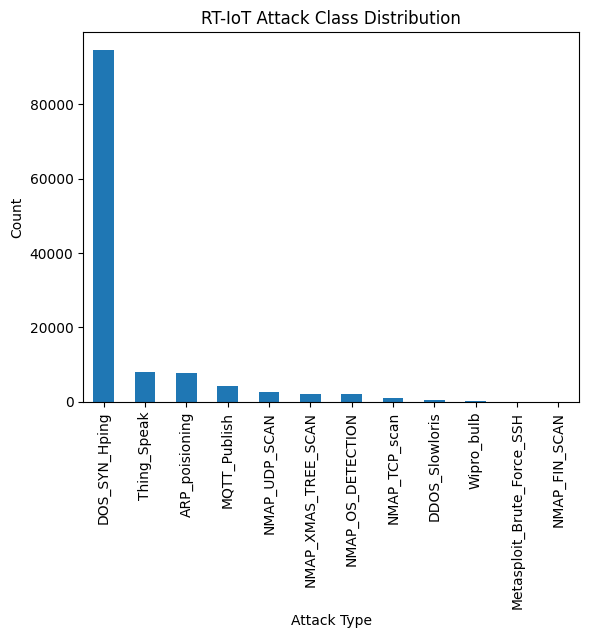
\includegraphics[keepaspectratio]{RT-IoT2022_files/figure-pdf/fig-rtiot-attack-dist-output-1.png}}

}

\caption{\label{fig-rtiot-attack-dist}RT-IoT attack class distribution}

\end{figure}%

\begin{longtable}[]{@{}lll@{}}

\caption{\label{tbl-rtiot-dtype-summary}Data type summary (excluding
target column)}

\tabularnewline

\toprule\noalign{}
& dtype & count \\
\midrule\noalign{}
\endhead
\bottomrule\noalign{}
\endlastfoot
0 & float64 & 47 \\
1 & int64 & 34 \\
2 & str & 2 \\

\end{longtable}

\begin{longtable}[]{@{}ll@{}}

\caption{\label{tbl-rtiot-string-features}String features in the
dataset}

\tabularnewline

\toprule\noalign{}
& string\_feature \\
\midrule\noalign{}
\endhead
\bottomrule\noalign{}
\endlastfoot
0 & proto \\
1 & service \\

\end{longtable}

\begin{longtable}[]{@{}lll@{}}

\caption{\label{tbl-rtiot-string-cardinality}String feature cardinality
summary}

\tabularnewline

\toprule\noalign{}
& feature & unique\_values \\
\midrule\noalign{}
\endhead
\bottomrule\noalign{}
\endlastfoot
0 & service & 10 \\
1 & proto & 3 \\

\end{longtable}

\begin{longtable}[]{@{}lll@{}}

\caption{\label{tbl-rtiot-skewness-filtered}Features exceeding skewness
threshold of 2.0 (absolute value)}

\tabularnewline

\toprule\noalign{}
& feature & abs\_skewness \\
\midrule\noalign{}
\endhead
\bottomrule\noalign{}
\endlastfoot
0 & bwd\_bulk\_bytes & 340.497528 \\
1 & bwd\_bulk\_packets & 340.490987 \\
2 & active.std & 287.992755 \\
3 & bwd\_pkts\_payload.tot & 280.814630 \\
4 & flow\_pkts\_payload.tot & 271.972274 \\
... & ... & ... \\
61 & flow\_FIN\_flag\_count & 5.127096 \\
62 & bwd\_init\_window\_size & 4.271062 \\
63 & flow\_pkts\_payload.std & 4.188075 \\
64 & flow\_pkts\_payload.min & 3.738574 \\
65 & fwd\_init\_window\_size & 2.785120 \\

\end{longtable}

\begin{figure}[H]

\centering{

\pandocbounded{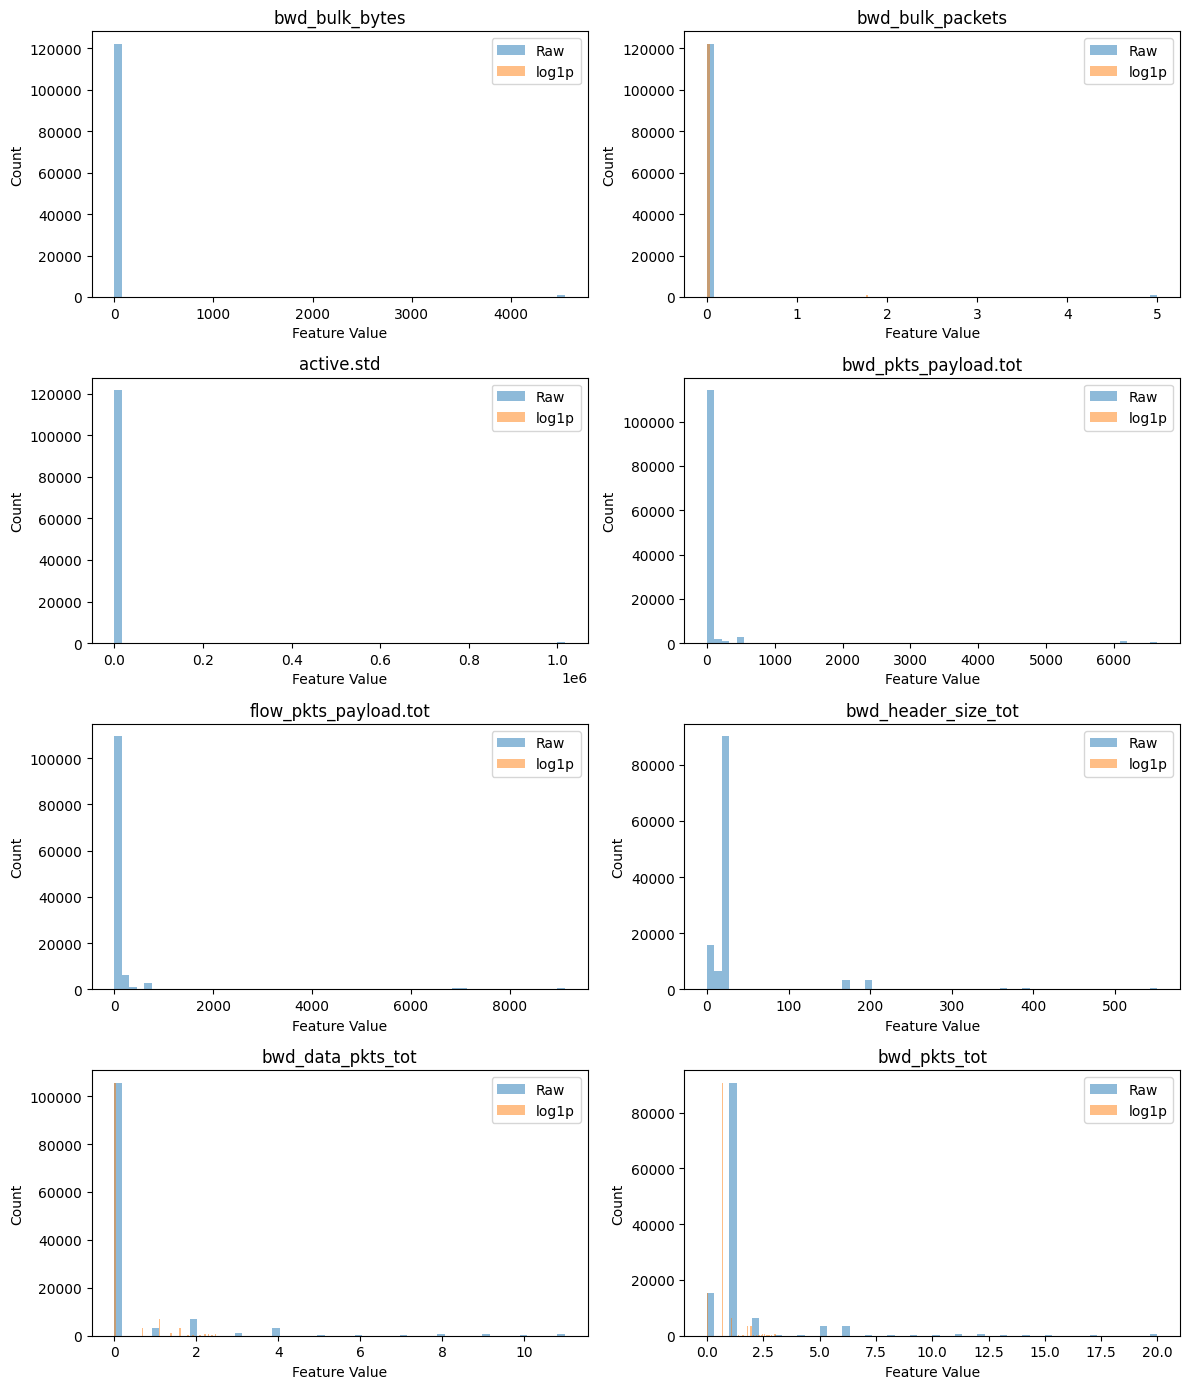
\includegraphics[keepaspectratio]{RT-IoT2022_files/figure-pdf/fig-rtiot-log-transform-justification-output-1.png}}

}

\caption{\label{fig-rtiot-log-transform-justification}Histogram
comparison of raw vs log-transformed distributions for the top 8 most
skewed features.}

\end{figure}%

\subsection{Identifying Class-Separating
Features}\label{identifying-class-separating-features}

To better understand which features distinguish normal and attack
traffic, we rank features using a \textbf{Standardized Mean Difference
(SMD)} measure aka Cohen's d, a filter-based feature selection approach
that quantifies class separability independent of model assumptions.

For each \textbf{numeric feature}, we compute a standardized difference
between the normal and attack distributions:

\[
d = \frac{|\mu_{\text{normal}} - \mu_{\text{attack}}|}{\sigma_{\text{pooled}}}
\]

where the pooled standard deviation summarizes variability across both
classes:

\[
\sigma_{\text{pooled}} =
\sqrt{\frac{\sigma_{\text{normal}}^{2} + \sigma_{\text{attack}}^{2}}{2}}
\]

And:

\begin{itemize}
\tightlist
\item
  \(\mu_{\text{normal}}\) --- mean feature value for normal traffic\\
\item
  \(\mu_{\text{attack}}\) --- mean feature value for attack traffic\\
\item
  \(\sigma_{\text{pooled}}\) --- pooled standard deviation across both
  classes\\
\item
  \(d\) --- standardized separation (effect size)
\end{itemize}

This metric quantifies how strongly a feature separates the two classes
independent of scale. Features with larger effect sizes indicate
\textbf{greater distributional separation between normal and attack
traffic} and are therefore more informative for visualization and
downstream modeling analysis.

The top-ranked features are selected as \textbf{class-separating
features} and used in the following exploratory visualizations.

\begin{longtable}[]{@{}lll@{}}

\caption{\label{tbl-rtiot-effect-sizes}Top 10 features by effect size
(numeric only)}

\tabularnewline

\toprule\noalign{}
& Features & Standardized Mean Difference \\
\midrule\noalign{}
\endhead
\bottomrule\noalign{}
\endlastfoot
0 & fwd\_pkts\_payload.min & 2.738131 \\
1 & fwd\_pkts\_payload.avg & 2.140473 \\
2 & fwd\_init\_window\_size & 1.666699 \\
3 & fwd\_pkts\_per\_sec & 1.493684 \\
4 & flow\_pkts\_per\_sec & 1.493501 \\
5 & bwd\_pkts\_per\_sec & 1.493306 \\
6 & bwd\_init\_window\_size & 1.471090 \\
7 & payload\_bytes\_per\_second & 1.435030 \\
8 & active.min & 1.054205 \\
9 & fwd\_subflow\_pkts & 0.965146 \\

\end{longtable}

\subsection{Analysis of Class-Separating
Features}\label{analysis-of-class-separating-features}

To better understand how normal and attack traffic differ, kernel
density estimates (KDEs) were plotted in Figure~\ref{fig-rtiot-kde} for
the top class-separating features identified using standardized mean
difference (SMD). These visualizations compare the empirical
distributions of normal and attack samples for each feature.

\begin{enumerate}
\def\labelenumi{\arabic{enumi}.}
\item
  Clear Distributional Separation:

  Across multiple features, attack traffic exhibits distinct statistical
  behavior compared to normal traffic. In particular:

  \begin{itemize}
  \tightlist
  \item
    Packet-rate features (\texttt{*\_pkts\_per\_sec},
    \texttt{flow\_pkts\_per\_sec}, \texttt{bwd\_pkts\_per\_sec}) show
    strong magnitude shifts between classes.
  \item
    Payload statistics (\texttt{fwd\_pkts\_payload.min},
    \texttt{fwd\_pkts\_payload.avg},
    \texttt{payload\_bytes\_per\_second}) demonstrate highly
    concentrated attack distributions with limited overlap.
  \item
    TCP window size features (\texttt{*\_init\_window\_size}) reveal
    substantially different operating ranges between normal and attack
    traffic.
  \item
    Flow activity and subflow metrics (\texttt{active.min},
    \texttt{fwd\_subflow\_pkts}) further distinguish attack behavior
    through tightly clustered value regions.
  \end{itemize}

  In many cases, the \textbf{attack distribution forms an extremely
  narrow peak while normal traffic remains broader and multimodal},
  indicating reduced variability within attack-generated flows.
\item
  Behavioral Differences in Network Traffic:

  The observed separation suggests that attacks modify fundamental
  traffic dynamics rather than subtle statistical properties.
  Specifically, attack flows tend to exhibit:

  \begin{itemize}
  \tightlist
  \item
    highly regular packet transmission rates,
  \item
    consistent payload characteristics,
  \item
    constrained TCP window configurations, and
  \item
    structured subflow behavior.
  \end{itemize}

  These patterns are consistent with \textbf{automated or scripted
  attack generation}, which produces repeatable traffic signatures
  compared to naturally varying user-driven network activity.
\item
  Low Overlap Between Classes:

  Several features display near-disjoint density regions, with attack
  samples concentrated within narrow intervals while normal traffic
  spans a wider range of values. This indicates that \textbf{individual
  features already encode strong discriminatory signal}, reducing
  reliance on complex feature interactions or nonlinear transformations
  for class separation.
\item
  Implications for Downstream Modeling:

  The presence of strong class separation at the feature level suggests
  that \textbf{linear decision boundaries may capture much of the
  discriminative structure} present in the dataset. Consequently, a
  simple supervised baseline model is well justified before introducing
  more complex representation-learning approaches such as autoencoders.

  Importantly, these findings reflect meaningful behavioral differences
  between normal and attack traffic patterns captured by the RT-IoT 2022
  dataset rather than evidence of data leakage.

  Overall, the exploratory analysis demonstrates that a subset of
  packet-rate, payload, window-size, and flow-activity features provides
  substantial statistical separation between classes. These results
  establish an empirical foundation for subsequent modeling experiments
  and help explain why relatively simple classifiers may achieve strong
  performance on this dataset.
\end{enumerate}

\begin{figure}[H]

\centering{

\pandocbounded{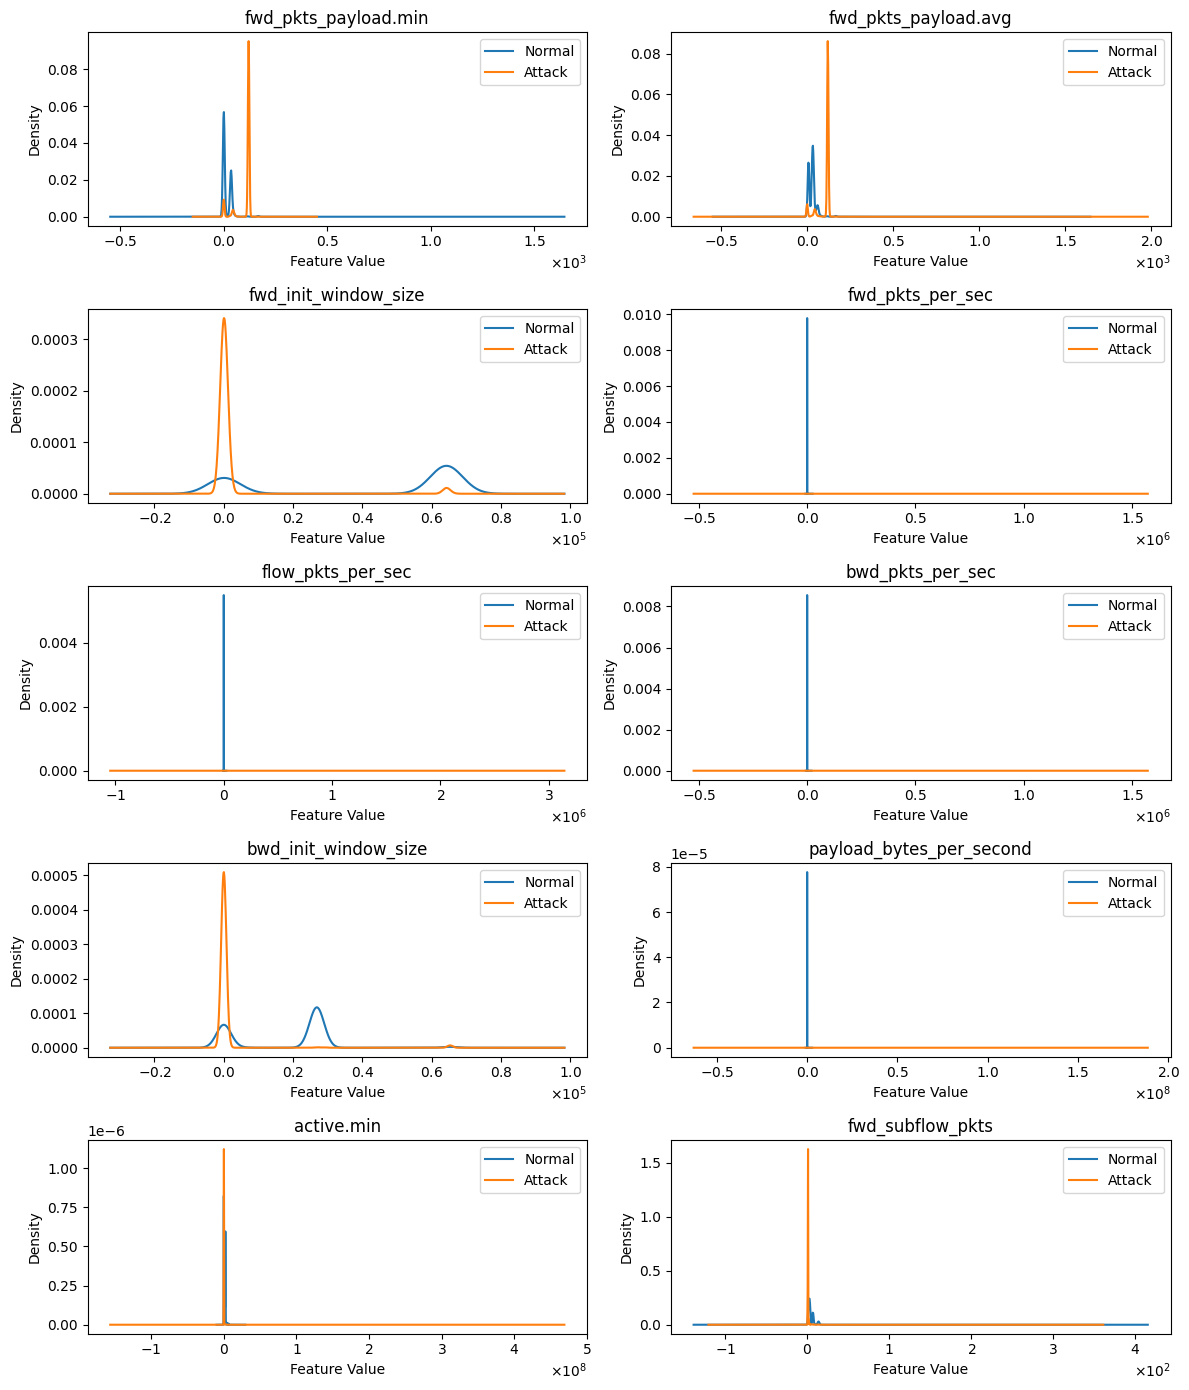
\includegraphics[keepaspectratio]{RT-IoT2022_files/figure-pdf/fig-rtiot-kde-output-1.png}}

}

\caption{\label{fig-rtiot-kde}KDE plots of top features by effect size}

\end{figure}%

\subsection{Correlation Structure of Top Class-Separating
Features}\label{correlation-structure-of-top-class-separating-features}

Figure~\ref{fig-rtiot-corr-heatmap} presents the Pearson correlation
matrix for the top class-separating numeric features identified during
exploratory analysis. The heatmap reveals several clear structural
patterns that provide insight into redundancy and behavioral groupings
within the RT-IoT 2022 dataset.

\begin{enumerate}
\def\labelenumi{\arabic{enumi}.}
\item
  \textbf{Strong Feature Clustering and Redundancy:}

  The most prominent observation is the presence of distinct
  \textbf{blocks of highly correlated features} (correlation
  coefficients approaching ±1). These clusters indicate that multiple
  variables capture closely related aspects of the same underlying
  network behavior rather than independent signals.

  In particular:

  \begin{itemize}
  \tightlist
  \item
    Packet-rate features (\texttt{*\_pkts\_per\_sec}) exhibit
    near-perfect positive correlation with one another, suggesting they
    are derived from common traffic counters.
  \item
    Inter-arrival time statistics (\texttt{flow\_iat.*},
    \texttt{fwd\_iat.*}, \texttt{idle.*}) form a dense correlation
    block, reflecting shared temporal characteristics of network flows.
  \item
    Payload and header-size measurements also display moderate-to-strong
    correlations, indicating overlapping representations of packet
    structure.
  \end{itemize}

  This redundancy implies that many high-ranking features encode similar
  information about traffic intensity and timing dynamics.
\item
  Behavioral Grouping of Network Characteristics:

  The correlation structure naturally separates features into
  interpretable behavioral categories:

  \begin{itemize}
  \tightlist
  \item
    \textbf{Transmission intensity:} packet rates and payload throughput
    metrics.
  \item
    \textbf{Temporal dynamics:} inter-arrival times, idle durations, and
    activity statistics.
  \item
    \textbf{Protocol and structural properties:} window sizes and
    header-related features.
  \end{itemize}

  These groupings suggest that attack behavior manifests through
  coordinated changes across multiple related measurements rather than
  isolated feature shifts.
\item
  \textbf{Limited Independence Among Top Predictors:} Relatively few
  features appear statistically independent. \textbf{High correlations
  indicate substantial multicollinearity}, meaning that including many
  correlated variables may not significantly increase predictive power
  but can \textbf{increase model complexity and computational cost}.
\item
  \textbf{Implications for Feature Selection and Modeling:} The observed
  correlation structure \textbf{supports the use of feature reduction}
  prior to deployment. Because many variables measure similar traffic
  properties, a smaller subset of representative features can likely
  preserve most predictive information while improving efficiency. For
  linear models such as Logistic Regression, correlated predictors are
  \textbf{partially mitigated through L2 regularization}; however,
  reducing redundancy remains \textbf{beneficial for interpretability
  and resource-constrained deployment} scenarios.
\item
  \textbf{Connection to Dataset Characteristics:} The clustered
  correlations reflect the engineered nature of network-flow datasets,
  where multiple statistics are computed from the same packet stream. As
  a result, \textbf{high correlation does not indicate noise but rather
  repeated measurements} of shared underlying traffic processes.
  Overall, the correlation analysis demonstrates that the RT-IoT 2022
  dataset contains strong but highly redundant signals, reinforcing the
  motivation for dimensionality reduction and efficient feature
  selection in subsequent modeling stages.
\end{enumerate}

\begin{figure}[H]

\centering{

\pandocbounded{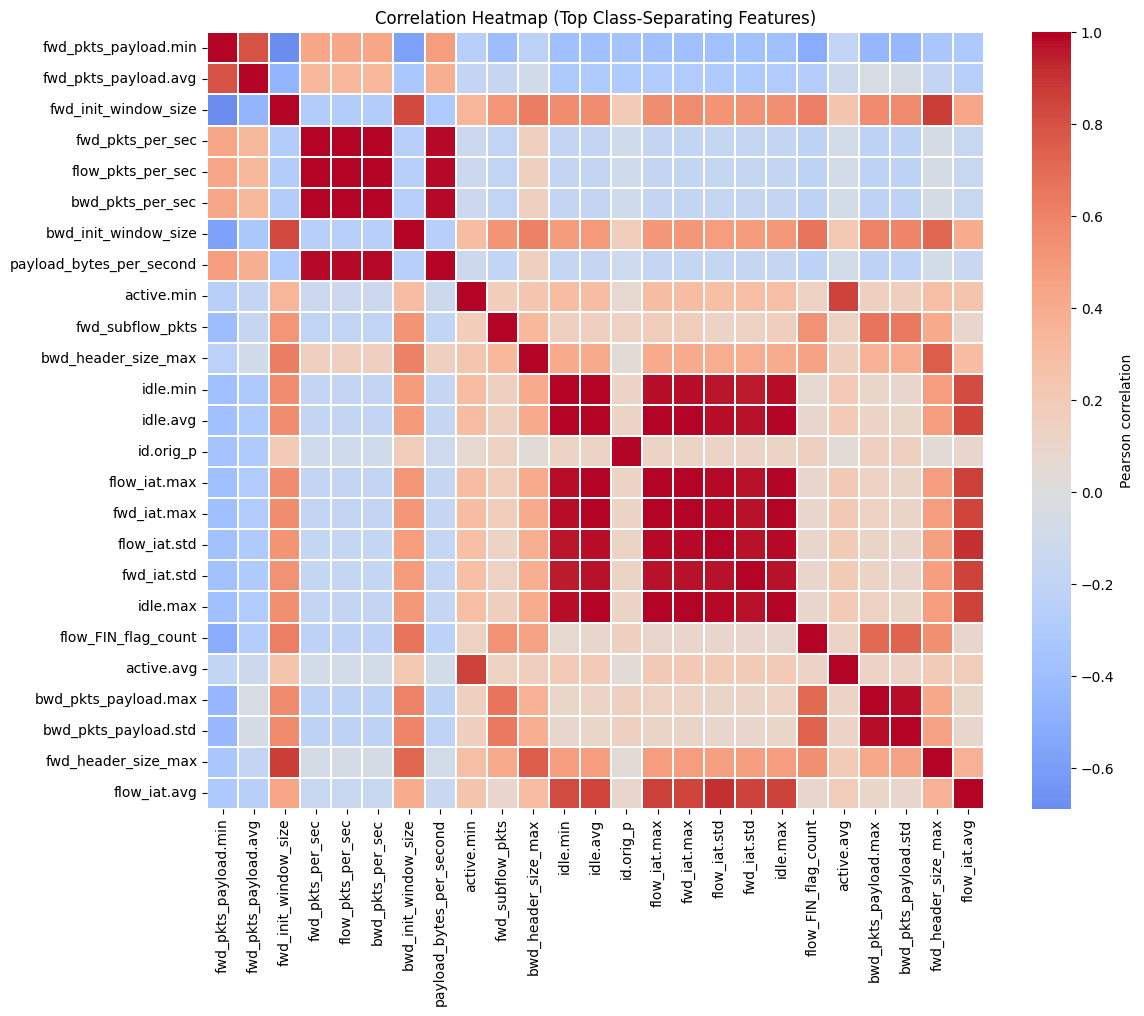
\includegraphics[keepaspectratio]{RT-IoT2022_files/figure-pdf/fig-rtiot-corr-heatmap-output-1.png}}

}

\caption{\label{fig-rtiot-corr-heatmap}Correlation heatmap of top
class-separating numeric features (by effect size)}

\end{figure}%

\subsection{Analysis of Top Features by Mutual
Information}\label{analysis-of-top-features-by-mutual-information}

To quantify the predictive relevance of individual variables,
\textbf{mutual information (MI)} was computed between each numeric
feature and the attack labels. Mutual information measures how much
knowing a feature reduces uncertainty about class membership, capturing
\textbf{both linear and nonlinear dependencies} between network traffic
characteristics and attack behavior.

Mutual information quantifies statistical dependence between a feature
\(X\) and the target variable \(y\):

\[
I(X;Y)=\sum_{x,y} p(x,y)\log\frac{p(x,y)}{p(x)p(y)}.
\]

It can also be interpreted as a reduction in uncertainty:

\[
I(X;Y)=H(Y)-H(Y|X),
\]

where \(H(Y)\) denotes entropy and \(H(Y|X)\) represents conditional
entropy. A value of \(I(X;Y)=0\) implies statistical independence
between \(X\) and \(Y\). Because mutual information captures both linear
and nonlinear relationships, it is well suited for network traffic
analysis, where attack behavior may alter packet statistics in complex,
non-linear ways.

The top eight features ranked by mutual information as shown in
Figure~\ref{fig-rtiot-mi} are:

\begin{itemize}
\tightlist
\item
  \texttt{fwd\_pkts\_payload.avg}
\item
  \texttt{fwd\_pkts\_payload.max}
\item
  \texttt{fwd\_subflow\_bytes}
\item
  \texttt{flow\_pkts\_payload.tot}
\item
  \texttt{fwd\_pkts\_payload.tot}
\item
  \texttt{flow\_pkts\_payload.avg}
\item
  \texttt{flow\_pkts\_payload.max}
\item
  \texttt{id.resp\_p}
\end{itemize}

\begin{enumerate}
\def\labelenumi{\arabic{enumi}.}
\item
  \textbf{Strong Predictive Signal at the Feature Level:}

  All top-ranked features exhibit exceptionally high mutual information
  scores (≈ 0.85), indicating that \textbf{individual variables alone
  provide substantial information} about whether a flow corresponds to
  normal or attack traffic. This suggests that class separation in the
  RT-IoT 2022 dataset arises primarily from clear behavioral differences
  rather than subtle multivariate interactions.

  Notably, most high-ranking variables are derived from \textbf{packet
  payload statistics}, including averages, maxima, and total payload
  sizes. These measurements capture how data is transmitted within flows
  and appear to differ systematically between normal and attack traffic.
\item
  \textbf{Dominance of Payload-Based Traffic Characteristics:}

  The concentration of payload-related features among the top predictors
  indicates that attacks modify fundamental transmission behavior.
  Compared to normal traffic, attack flows tend to exhibit:

  \begin{itemize}
  \tightlist
  \item
    more consistent payload magnitudes,
  \item
    structured packet generation patterns,
  \item
    and reduced variability across packets within a flow.
  \end{itemize}

  Such regularity is characteristic of automated attack tools, which
  generate traffic programmatically rather than through organic
  user-driven interactions.
\item
  \textbf{Evidence of Feature Redundancy:}

  Several top features \textbf{measure closely related quantities}
  (e.g., average, maximum, and total payload statistics). While each
  individually shows strong predictive power, their similarity suggests
  substantial redundancy. This implies that increasing the number of
  included features beyond the highest-ranked subset may provide
  diminishing returns, as additional variables often encode overlapping
  information about the same traffic behavior.
\item
  \textbf{Role of Network Context Features:}

  The inclusion of \texttt{id.resp\_p} among the top predictors
  highlights the importance of network context alongside payload
  statistics. \textbf{Port information implicitly captures service-level
  behavior}, indicating that certain attack patterns are associated with
  specific communication protocols.
\item
  \textbf{Implications for Downstream Modeling:}

  The presence of highly informative individual features explains the
  strong performance observed with linear classifiers such as Logistic
  Regression. Because \textbf{substantial class separation exists at the
  feature level}, complex nonlinear models are not strictly required to
  achieve strong discrimination performance.

  From a practical standpoint, these findings suggest that a
  \textbf{compact subset of high-MI features may be sufficient for
  effective intrusion detection while reducing computational cost}. This
  observation is particularly relevant for subsequent deployment
  experiments targeting resource-constrained environments such as
  Raspberry Pi devices.

  Overall, mutual information analysis demonstrates that payload
  dynamics and flow-level transmission characteristics form the primary
  statistical signature distinguishing normal and attack traffic within
  the RT-IoT 2022 dataset.
\end{enumerate}

\begin{figure}[H]

\centering{

\pandocbounded{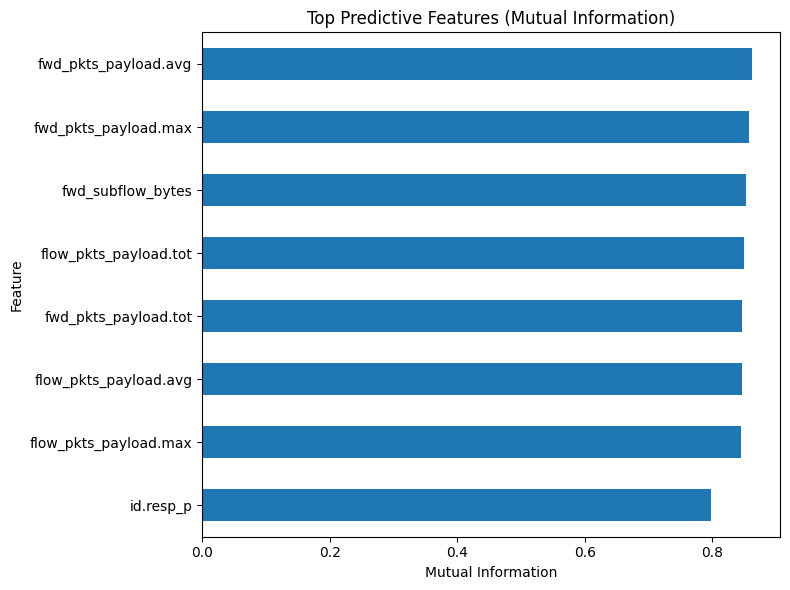
\includegraphics[keepaspectratio]{RT-IoT2022_files/figure-pdf/fig-rtiot-mi-output-1.png}}

}

\caption{\label{fig-rtiot-mi}Top 8 features ranked by mutual information
with the target label.}

\end{figure}%

\subsection{PCA Analysis}\label{pca-analysis}

\begin{enumerate}
\def\labelenumi{\arabic{enumi}.}
\item
  The two-dimensional PCA projection in Figure~\ref{fig-rtiot-pca} shows
  partial separation between normal and attack traffic but with
  substantial overlap, indicating that the classes are \textbf{not
  linearly separable in low-dimensional space}. Normal traffic appears
  more concentrated, while attack samples exhibit greater dispersion and
  several extreme outliers, suggesting \textbf{higher variability in
  malicious network behavior}. This pattern supports the anomaly
  detection assumption that normal traffic follows more structured
  patterns whereas attacks deviate from learned behavior.
\item
  The cumulative explained variance analysis in
  Figure~\ref{fig-rtiot-pca-variance} indicates that \textbf{the dataset
  is intrinsically high-dimensional}. Although the first two principal
  components capture only about 31\% of total variance,
  \textbf{approximately 20--30 components explain over 90--95\% of the
  variance}. This suggests strong redundancy among features and implies
  that meaningful structure exists in a moderately compressed latent
  space, providing justification for dimensionality reduction and
  representation-learning approaches such as autoencoders.
\end{enumerate}

\begin{figure}[H]

\centering{

\pandocbounded{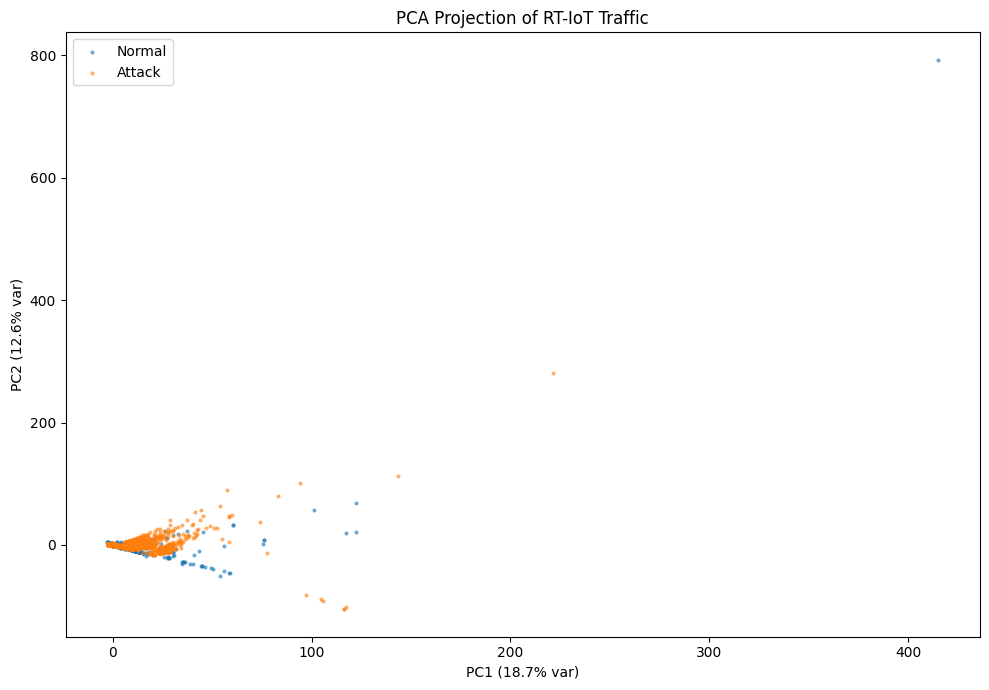
\includegraphics[keepaspectratio]{RT-IoT2022_files/figure-pdf/fig-rtiot-pca-output-1.png}}

}

\caption{\label{fig-rtiot-pca}PCA projection of RT-IoT traffic (2D)
colored by normal vs attack classes. Explained variance ratios for PC1
and PC2 are indicated in the axis labels.}

\end{figure}%

\begin{figure}[H]

\centering{

\pandocbounded{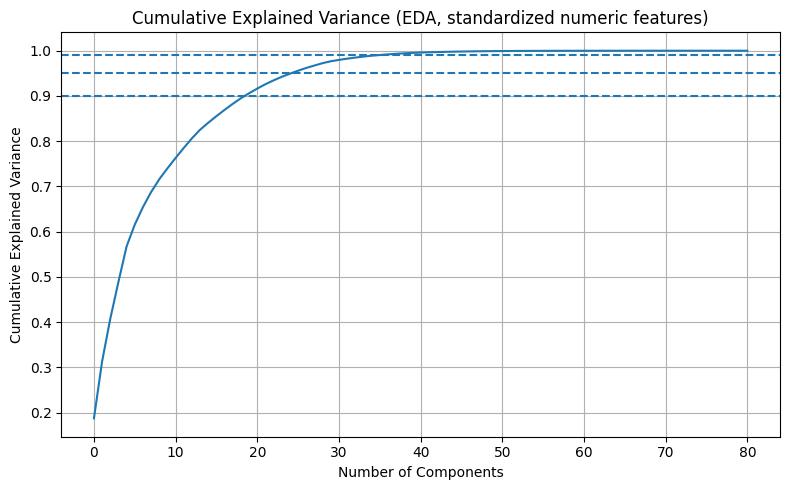
\includegraphics[keepaspectratio]{RT-IoT2022_files/figure-pdf/fig-rtiot-pca-variance-output-1.png}}

}

\caption{\label{fig-rtiot-pca-variance}Cumulative explained variance of
RT-IoT traffic features. Horizontal dashed lines indicate common
thresholds (90\%, 95\%, 99\%) for intrinsic dimensionality estimation.}

\end{figure}%

\section{Logistic Regression
Preprocessing:}\label{logistic-regression-preprocessing}

\subsection{Create binary label
(y\_bin):}\label{create-binary-label-y_bin}

For our baseline logistic regression, we will encode our multi-class
attack types into binary. - Converts multiclass Attack\_type into
binary: 0 = normal, 1 = attack - Normal classes are the benign IoT
device activity buckets: Thing\_Speak, MQTT\_Publish, and Wipro\_bulb

\begin{verbatim}
Binary label distribution (0=normal, 1=attack):
\end{verbatim}

\begin{longtable}[]{@{}lll@{}}

\caption{\label{tbl-rtiot-lr-binary}Binary label distribution (0=normal,
1=attack)}

\tabularnewline

\toprule\noalign{}
& count & rate \\
class & & \\
\midrule\noalign{}
\endhead
\bottomrule\noalign{}
\endlastfoot
0 & 12507 & 0.101586 \\
1 & 110610 & 0.898414 \\

\end{longtable}

\subsection{Check for duplicate rows and
remove:}\label{check-for-duplicate-rows-and-remove}

\begin{verbatim}
Rows removed: 5195
\end{verbatim}

\begin{longtable}[]{@{}llll@{}}

\caption{\label{tbl-rtiot-lr-deduplication}Deuplicate row summary for
RT-IoT dataset}

\tabularnewline

\toprule\noalign{}
& n\_rows & duplicate\_rows & duplicate\_rate \\
\midrule\noalign{}
\endhead
\bottomrule\noalign{}
\endlastfoot
0 & 117922 & 7 & 0.000059 \\

\end{longtable}

\subsection{Downsampling of Attack
Traffic:}\label{downsampling-of-attack-traffic}

The RT-IoT dataset exhibited substantial class imbalance due to the
absence of a large subset of normal traffic observations (Amazon-Alexa).
To prevent the classifier from learning a trivial majority-class
decision rule, we constructed a balanced training dataset using random
downsampling of the majority class.

Specifically, all normal traffic samples were retained, and an equal
number of attack observations were randomly selected without replacement
from the larger attack class. This procedure produced a 1:1 class ratio
while preserving only authentic network flows, avoiding the introduction
of synthetic data that could distort traffic distributions.

Downsampling was performed prior to the train--test split to ensure that
duplicated or highly similar attack flows were not unevenly distributed
across evaluation partitions. The resulting balanced dataset enables
fair comparison of model performance by reducing bias toward the
majority class and encouraging the model to learn discriminative
patterns between normal and malicious network behavior.

\begin{verbatim}
Balanced label distribution after downsampling (0=normal, 1=attack):
\end{verbatim}

\begin{longtable}[]{@{}lll@{}}

\caption{\label{tbl-rtiot-lr-balanced}Balanced dataset distribution
(after downsampling attacks)}

\tabularnewline

\toprule\noalign{}
& count & rate \\
class & & \\
\midrule\noalign{}
\endhead
\bottomrule\noalign{}
\endlastfoot
0 & 12015 & 0.5 \\
1 & 12015 & 0.5 \\

\end{longtable}

\subsection{Split train \& test (80/20)}\label{split-train-test-8020}

\begin{table}[H]

\caption{\label{tbl-rtiot-lr-split}Train/test split distribution for
target (balanced dataset)}

\centering{

\begin{verbatim}
Target train distribution: {1: 9612, 0: 9612}
Target test distribution: {0: 2403, 1: 2403}
\end{verbatim}

}

\end{table}%

\subsection{Baseline Model: Logistic
Regression}\label{baseline-model-logistic-regression}

\subsubsection{Motivation}\label{motivation}

Before evaluating more complex models such as autoencoders, we establish
a \textbf{supervised baseline classifier} using Logistic Regression.
This model provides a strong statistical reference point because it is:

\begin{itemize}
\tightlist
\item
  Interpretable
\item
  Computationally efficient
\item
  Well-understood theoretically
\item
  A standard benchmark for tabular classification problems
\end{itemize}

The purpose of this baseline is to measure how well a classical linear
model can distinguish between \textbf{normal} and \textbf{attack}
network traffic in the RT-IoT 2022 dataset.

\subsubsection{Model Formulation}\label{model-formulation}

Logistic Regression models the probability that an observation belongs
to the attack class given a feature vector \(x \in \mathbb{R}^d\). The
model assumes a linear relationship between features and the log-odds of
the outcome:

\[
P(y = 1 \mid x) = \sigma(w^\top x + b)
\]

where

\[
\sigma(z) = \frac{1}{1 + e^{-z}}
\]

is the sigmoid function, (w) represents model coefficients, and (b) is
the intercept.

Equivalently, Logistic Regression models the log-odds (logit) as a
linear function:

\[
\log \frac{P(y=1 \mid x)}{P(y=0 \mid x)} = w^\top x + b
\]

\subsubsection{Optimization Objective}\label{optimization-objective}

Model parameters are learned by minimizing the \textbf{regularized
negative log-likelihood} (logistic loss):

\[
\mathcal{L}(w,b)
=
-\frac{1}{n}
\sum_{i=1}^{n}
\left[
y_i \log(p_i) + (1-y_i)\log(1-p_i)
\right]
+ \lambda \|w\|_2^2
\]

where

\[
p_i = \sigma(w^\top x_i + b)
\]

and \(\lambda \|w\|_2^2\) represents L2 regularization, which
discourages excessively large coefficients and improves generalization.

The optimization is solved numerically using gradient-based methods
(LBFGS in scikit-learn).

\subsubsection{Implementation}\label{implementation}

The baseline model is implemented using scikit-learn's
\texttt{Pipeline}, which integrates preprocessing and classification
into a single reproducible workflow. All preprocessing steps are learned
exclusively from the training data within each cross-validation fold,
preventing information leakage during model evaluation.

The pipeline consists of the following components:

\begin{itemize}
\item
  \textbf{Categorical encoding:} the \texttt{proto} and \texttt{service}
  variables are transformed using \textbf{one-hot encoding}, converting
  categorical network descriptors into mutually exclusive binary
  indicator features. The encoder is fit only on the training split,
  ensuring consistent feature mappings and safe handling of unseen
  categories during evaluation.
\item
  \textbf{Log transformation of skewed features:} numeric predictors
  exhibiting strong distributional asymmetry (\textbf{absolute skewness
  greater than 2.0}, identified during exploratory analysis) are
  transformed using the \(\log(1+x)\) function. This
  variance-stabilizing transformation reduces heavy-tailed behavior
  common in network traffic statistics and mitigates the influence of
  extreme flow values on model estimation.
\item
  \textbf{Feature standardization:} following transformation, all
  numeric features are standardized using \texttt{StandardScaler}.
  Scaling ensures comparable feature magnitudes and improves numerical
  stability during optimization.
\item
  \textbf{Logistic Regression classifier:} a regularized Logistic
  Regression model (\texttt{solver="lbfgs"}) estimates class
  probabilities using an \textbf{L2 penalty} to control coefficient
  magnitude and improve generalization.
\end{itemize}

Encapsulating encoding, transformation, scaling, and classification
within a single pipeline guarantees that preprocessing is recomputed
independently for each cross-validation split. This produces leak-free
out-of-fold predictions while maintaining identical preprocessing during
training and testing. Using a unified pipeline also enables \textbf{fair
comparison with subsequent models} by enforcing a consistent
experimental framework across experiments. Consequently, observed
performance differences reflect modeling choices rather than
inconsistencies in data preparation.

\subsubsection{Evaluation:}\label{evaluation}

After training the Logistic Regression model and calibrating the
decision threshold using out-of-fold predictions on the training data,
we perform a \textbf{single final evaluation} on the held-out test set.
This step provides an unbiased estimate of real-world performance
because:

\begin{itemize}
\tightlist
\item
  The model was trained only on training data.
\item
  The classification threshold was tuned using cross-validation.
\item
  The test set remains completely unseen until this stage.
\end{itemize}

This separation prevents information leakage and ensures statistically
valid evaluation.

\subsection{Logistic Regression Baseline: Key Findings
(WORKING)}\label{logistic-regression-baseline-key-findings-working}

Table~\ref{tbl-rtiot-lr-cv-summary} Table~\ref{tbl-rtiot-lr-test-eval}
Table~\ref{tbl-rtiot-lr-confusion-matrix} Figure~\ref{fig-rtiot-lr-roc}
Table~\ref{tbl-rtiot-lr-coefs}

\begin{longtable}[]{@{}llll@{}}

\caption{\label{tbl-rtiot-lr-cv-summary}Logistic Regression
Cross-Validation Summary showing best threshold and corresponding F1
score on out-of-fold predictions (train-only).}

\tabularnewline

\toprule\noalign{}
& best\_threshold & best\_oof\_f1\_attack & cv\_folds \\
\midrule\noalign{}
\endhead
\bottomrule\noalign{}
\endlastfoot
0 & 0.458 & 0.994481 & 5 \\

\end{longtable}

\begin{longtable}[]{@{}ll@{}}

\caption{\label{tbl-rtiot-lr-test-eval}Test set evaluation metrics for
Logistic Regression baseline at tuned threshold from train-only
cross-validation.}

\tabularnewline

\toprule\noalign{}
& value \\
\midrule\noalign{}
\endhead
\bottomrule\noalign{}
\endlastfoot
threshold & 0.458000 \\
precision\_attack & 0.993347 \\
recall\_attack & 0.994174 \\
f1\_attack & 0.993760 \\
f1\_macro & 0.993758 \\
roc\_auc & 0.999260 \\
pr\_auc & 0.999204 \\
tn & 2387.000000 \\
fp & 16.000000 \\
fn & 14.000000 \\
tp & 2389.000000 \\

\end{longtable}

\begin{longtable}[]{@{}lll@{}}

\caption{\label{tbl-rtiot-lr-confusion-matrix}Confusion Matrix for
Logistic Regression at tuned threshold.}

\tabularnewline

\toprule\noalign{}
& pred\_normal(0) & pred\_attack(1) \\
\midrule\noalign{}
\endhead
\bottomrule\noalign{}
\endlastfoot
true\_normal(0) & 2387 & 16 \\
true\_attack(1) & 14 & 2389 \\

\end{longtable}

\begin{verbatim}
ROC curve (test set)
\end{verbatim}

\begin{figure}[H]

\centering{

\pandocbounded{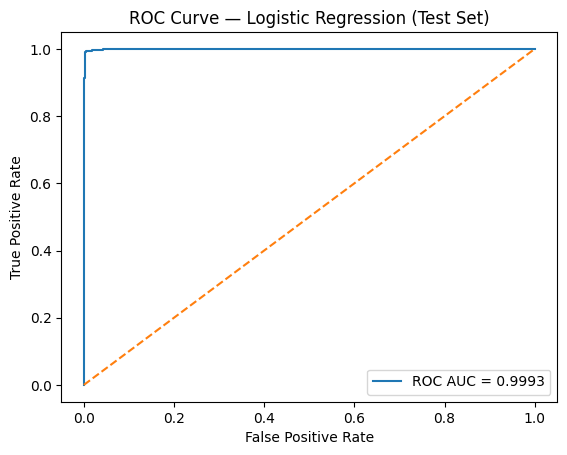
\includegraphics[keepaspectratio]{RT-IoT2022_files/figure-pdf/fig-rtiot-lr-roc-output-2.png}}

}

\caption{\label{fig-rtiot-lr-roc}ROC curve for Logistic Regression on
test set, showing AUC score.}

\end{figure}%

\begin{longtable}[]{@{}lll@{}}

\caption{\label{tbl-rtiot-lr-coefs}Top 8 features by absolute
coefficient magnitude from Logistic Regression model, indicating their
relative importance for attack detection.}

\tabularnewline

\toprule\noalign{}
& feature & abs\_coefficient \\
\midrule\noalign{}
\endhead
\bottomrule\noalign{}
\endlastfoot
0 & flow\_ACK\_flag\_count & 3.920119 \\
1 & service\_mqtt & 3.864157 \\
2 & fwd\_header\_size\_max & 2.618150 \\
3 & bwd\_subflow\_pkts & 2.326884 \\
4 & flow\_ECE\_flag\_count & 2.294272 \\
5 & bwd\_pkts\_payload.max & 2.281785 \\
6 & fwd\_init\_window\_size & 2.264444 \\
7 & fwd\_subflow\_bytes & 2.187293 \\
8 & fwd\_iat.tot & 2.105937 \\
9 & active.std & 2.050897 \\
10 & id.orig\_p & 1.858290 \\
11 & idle.max & 1.747019 \\
12 & service\_- & 1.732238 \\
13 & bwd\_pkts\_tot & 1.709193 \\
14 & fwd\_data\_pkts\_tot & 1.671155 \\
15 & idle.min & 1.633192 \\
16 & service\_dns & 1.603858 \\
17 & flow\_pkts\_per\_sec & 1.565167 \\
18 & bwd\_pkts\_payload.min & 1.535344 \\
19 & fwd\_iat.std & 1.456755 \\

\end{longtable}

\section{Next Steps:}\label{next-steps}

\begin{enumerate}
\def\labelenumi{\arabic{enumi})}
\tightlist
\item
  Model Selection
\item
  Autoencoder baseline
\item
  QAE models
\item
  Raspberry pie model implementation
\item
  Metrics collection + analysis
\end{enumerate}




\end{document}
